\documentclass[10pt]{beamer}
\usepackage{bbm}
\usepackage{fontspec}

\usepackage{mathtools}
\usepackage{graphicx}
\usepackage{animate}
\renewcommand\appendixname{Appendix}
\usepackage{xcolor}
\usepackage{tikz}
\colorlet{rred}{red!80!black}
\colorlet{ggreen}{green!80!black}
\colorlet{grey}{black!50!white}




\usetheme[progressbar=foot]{metropolis}
\usepackage{appendixnumberbeamer}
\setbeamercovered{dynamic}

\usepackage{booktabs}
\usepackage[scale=2]{ccicons}

\usepackage{pgfplots}
\usepgfplotslibrary{dateplot}
\setbeamertemplate{caption}{\raggedright\insertcaption\par}
\setlength{\abovecaptionskip}{-10pt plus 0pt minus 0pt}

\usepackage{xspace}
\newcommand{\themename}{\textbf{\textsc{metropolis}}\xspace}
\theoremstyle{definition}
\newtheorem{defn}{Definition}
\newtheorem{obs}{Observation}

% math symbols
\newcommand{\R}{\mathbb{R}}
\newcommand{\N}{\mathbb{N}}
\newcommand{\Z}{\mathbb{Z}}
\newcommand{\E}{\mathbb{E}}
\newcommand{\HBB}{\mathbb{H}}
\newcommand{\1}{\mathbbm{1}}
\newcommand{\XX}{\mathcal{X}}
\newcommand{\TT}{\mathcal{T}}
\newcommand{\YY}{\mathcal{Y}}
\newcommand{\UU}{\mathcal{U}}
\newcommand{\VV}{\mathcal{V}}
\newcommand{\WW}{\mathcal{W}}
\newcommand{\LL}{\mathcal{L}}
\newcommand{\PP}{\mathcal{P}}
\newcommand{\QQ}{\mathcal{Q}}
\DeclareMathOperator*{\argmin}{argmin}
\DeclareMathOperator*{\argmax}{argmax}
\title{Stochastic Neighborhood Embedding}
\subtitle{Weekly AI pills}
\date{2020-11-13}
\author{Fabio Brau.}
\institute{SSSA, Emerging Digital Technologies, Pisa.}
% \titlegraphic{\hfill\includegraphics[height=1.5cm]{logo.pdf}}

\usebackgroundtemplate{%
    \begin{picture}(300,271)
      \hspace{11.2cm}
       
\includegraphics[scale=0.1]{pic/logoretis_noname.png}
   \end{picture}}

\begin{document}
{\usebackgroundtemplate{%
    \begin{picture}(300,265)
      \hspace{0.9cm}
       
\includegraphics[scale=0.5]{pic/tecip_logo.png}
       \hspace{0.5cm}
       
\includegraphics[scale=0.21]{pic/logoretis_320.png}
   \end{picture}}%
\maketitle
}
\begin{frame}{Summary}
  \begin{enumerate}
    \item Entropy and Kullback–Leibler divergence
    \item From SNE to t-SNE
    \item Application for Visualization
    \item Issues
  \end{enumerate}
\end{frame}
\begin{frame}{Introduction}{}
%  {\bf Main Papers}\\
%    Stochastic Neighbor Embedding - Hinton \& Roweis - 2002\\
%    Visualizing Data using t-SNE - Maaten \& Hinton - 2008\\
%    \vfill
  \begin{center}
    (t)-{\bf S}tochastic {\bf N}eighborhood {\bf E}mbedding
  \end{center}
  \begin{minipage}{0.4\textwidth}
    {\bf Aims}
    \begin{itemize}
      \item Dimensionality Reduction
      \item Data Visualization
        \begin{enumerate}
          \item Exploration
          \item Visual Clustering
        \end{enumerate}
    \end{itemize}
  \end{minipage}\hfill
  \begin{minipage}{0.4\textwidth}
    \begin{figure}[h!]
      \centering
      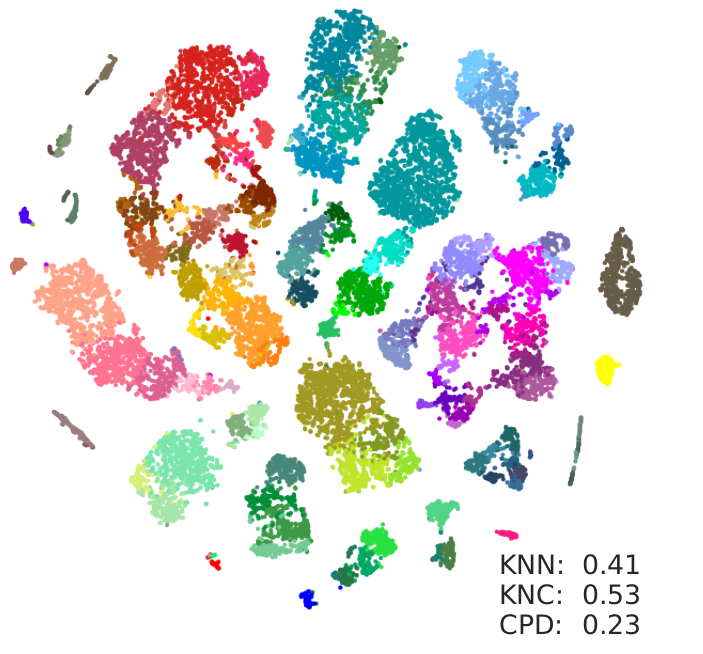
\includegraphics[scale=0.2]{./pic/example.png}
      \caption{Example of Data Visualization taken from (Tasic et al., 2018)}
    \end{figure}
  \end{minipage} 
\end{frame}
\section{Algorithm}
\begin{frame}{Algorithm: Workflow}
  \begin{enumerate}
    \item Represent each sample $x_i \in\XX$ with $y_i\in\YY$ in a
      low-dimensional space
      \[
        \Phi :
        \underset{\subseteq \R^n}{\XX} \longrightarrow
        \underset{\subseteq \R^2}{\YY}
    \]
    \item Convert {\bf Geometrical Information} to {\bf Probabilistic
      Distribution} 
      \[
        \begin{aligned}
          p_{i|j} : \mbox{``Probability that $x_i$ is {\it\color{gray}
          similar} to $x_j$'' }\\
          q_{i|j} : \mbox{``Probability that $y_i$ is {\it\color{gray}
          similar} to $y_j$'' }
        \end{aligned}
      \]
    \item Compare distribution $\PP$ of $\XX$ to distribution $\QQ$ of $\XX$
    \item Adjust the representation $\Phi$ to make distributions closer.
  \end{enumerate}
  \onslide<2->
  \begin{obs}
    The embedding $\Phi$ is defined {\bf point-wise}, i.e $\Phi$ is only defined over
    $\XX$ through the definition $\Phi(x_i) = y_i$. Another way to say
    ``$y_i$ are the parameters of $\Phi$'' (Future works?).
  \end{obs}
\end{frame}
\begin{frame}{Algorithm: Similarity and Probability Distribution}
  \begin{defn}[Similarity with Gaussian Kernel]
    \vspace{1px}
    For each $x_i$ we fix a $\sigma_i$ and define
    \begin{equation}
      \forall j\ne i,\quad p_{i|j}  = \frac{\exp\left(-\|x_i -
      x_j\|^2/(2\sigma_i)^2\right)}{\sum_{k\ne i}\exp\left(-\|x_i - x_k\|^2 /
    (2\sigma_i)^2\right)}
      \tag{$\PP_i$}
    \end{equation}
  \end{defn}
  \onslide<2->
    {\bf How $\sigma_i$ impacts?}
  \begin{figure}[h!]
    \centering
    \includegraphics<2>[scale=0.4, trim=0 0 0 1cm]{{pic/similarity_0.1}.pdf}%
    \includegraphics<3>[scale=0.4, trim=0 0 0 1cm]{{pic/similarity_0.2}.pdf}%
    \includegraphics<4>[scale=0.4, trim=0 0 0 1cm]{{pic/similarity_0.5}.pdf}%
    \includegraphics<5>[scale=0.4, trim=0 0 0 1cm]{{pic/similarity_1.0}.pdf}%
    \includegraphics<6->[scale=0.4, trim=0 0 0 1cm]{{pic/similarity_2.0}.pdf}%
  \end{figure}
\end{frame}
\begin{frame}{Algorithm: Similarity and Probability Distribution}
  At the same manner we can define similarity in $\YY$.
  \begin{equation}
    \forall j\ne i,\quad q_{i|j}  = \frac{\exp\left(-\|y_i -
    y_j\|^2\right)}{\sum_{k\ne i}\exp\left(-\|y_i - y_k\|^2\right)}
    \tag{$\QQ_i$}
  \end{equation}
  \vfill
  {\bf Observation}\\
  $\PP_i$ and $\QQ_i$ are probability distributions  for each $i$.
  \begin{enumerate}
  \item $0 \le p_{i|j},q_{i|j} \le 1$ for each $j\ne i$
  \item $\sum_{j\ne i} p_{i|j} = \sum_{j\ne i} q_{i|j} = 1 $
\end{enumerate}
\end{frame}
\begin{frame}{Shannon Entropy, Perplexity, Kullback–Leibler Divergence}{}
  %{\it ``The Entropy measures the complexity of the information''}\\
  \vfill
  Let $ \PP=\{p_1, \cdots, p_n\}$ and $\QQ=\{q_1,\cdots,q_n\}$  distributions
  \begin{equation*}
    \begin{aligned}
      \mbox{\bf Shannon Entropy}\qquad &\HBB(\PP) =
      -\sum_i p_i\log_2(p_i)\\
      \mbox{\bf Perplexity} \qquad & Perp(\PP) = 2^{\HBB(\PP)}\\
      \mbox{\bf K.L. Divergence} \qquad & KL(\PP,\QQ) = \sum_i
      p_i\log_2\left( \frac{p_i}{q_i} \right)\\
    \end{aligned}
    \label{entropy}
  \end{equation*}
  \begin{minipage}[h!]{\textwidth}
    {\bf How $\sigma_i$ and Perplexity are related?}
    \begin{figure}[h!]
      \centering
      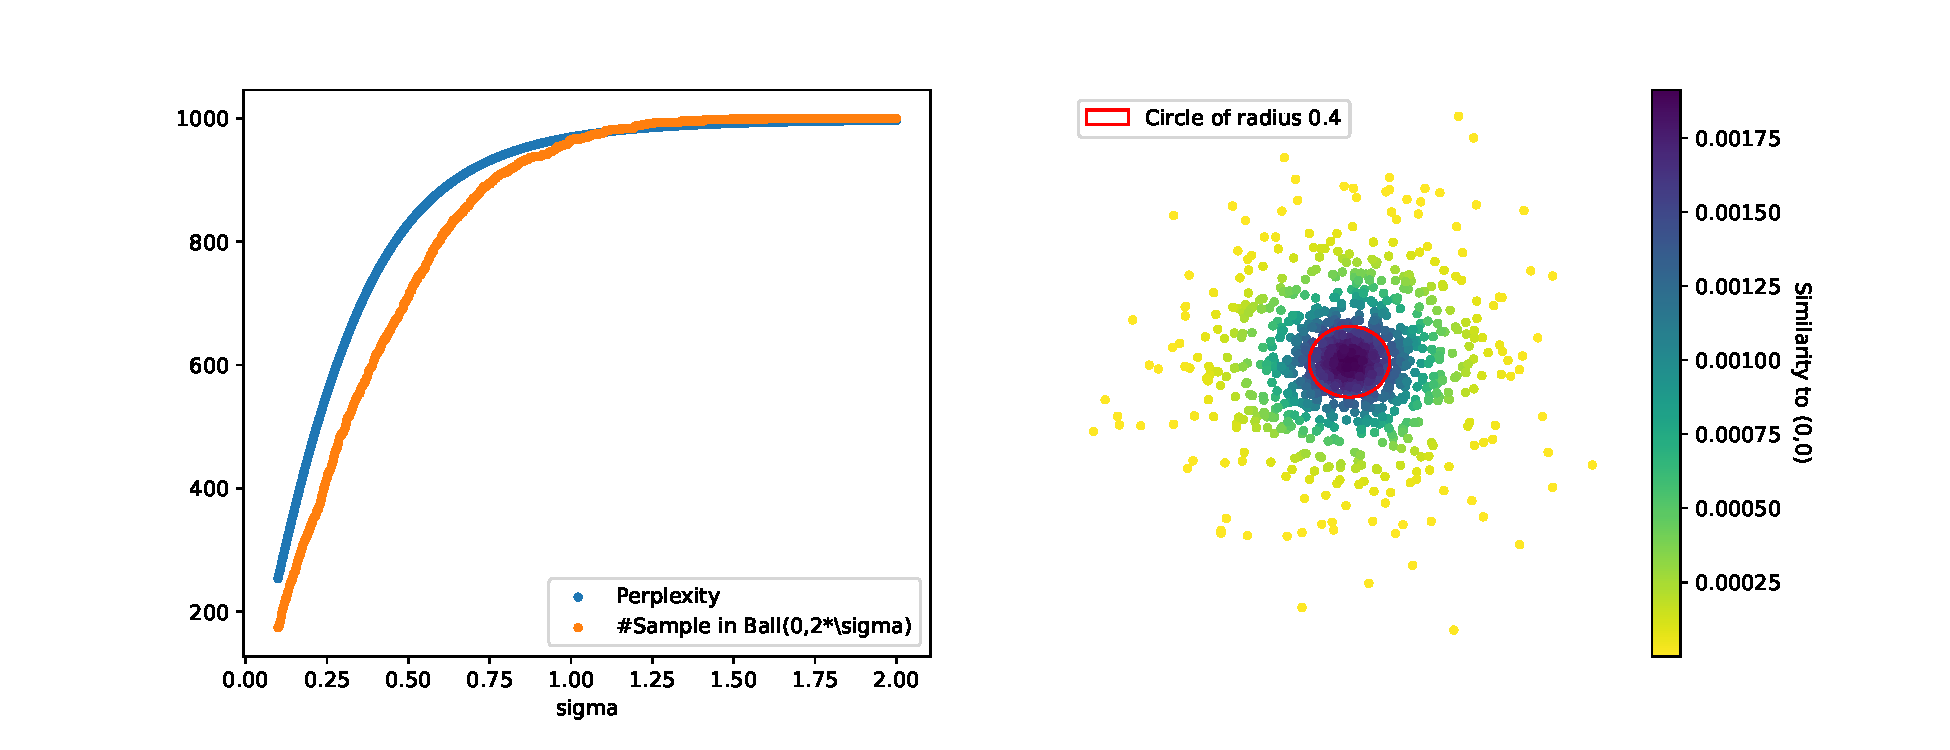
\includegraphics[clip, scale=0.32, trim=0 0 0
      1cm]{./pic/perplexity.pdf}
      \caption{Perplexity measures the number of samples in a neighborhood.}
    \end{figure}
  \end{minipage}
\end{frame}
\end{document}

